\begin{table*}[t!]
\caption{\textbf{Learning from pixels.} Return of our method (TD-MPC) and state-of-the-art algorithms on the image-based DMControl 100k benchmark used in \citet{srinivas2020curl, kostrikov2020image, Ye2021MasteringAG}. Baselines are tuned specifically for image-based RL, whereas our method is not. Results for SAC, CURL, DrQ, and PlaNet are partially obtained from \citet{srinivas2020curl, kostrikov2020image}, and results for Dreamer, MuZero, and EfficientZero are obtained from \citet{Hafner2020DreamTC, Ye2021MasteringAG}. Mean and std. deviation over 10 runs. \textbf{*}: MuZero and EfficientZero use a discretized action space, and EfficientZero performs an additional 20k gradient steps before evaluation, whereas other methods do not. Due to dimensionality explosion under discretization, MuZero and EfficientZero cannot feasibly solve tasks with higher-dimensional action spaces, e.g., Walker Walk and Cheetah Run ($\mathcal{A} \in \mathbb{R}^{6}$), while our method can.}
\label{tab:planet}
\vspace{0.05in}
\centering
\resizebox{0.91\textwidth}{!}{%
\begin{tabular}{lcccc|cccc|c}
\multicolumn{1}{c}{} & \multicolumn{4}{c}{Model-free} & \multicolumn{4}{c}{Model-based} & \multicolumn{1}{c}{Ours} \\
\toprule
\textit{100k env. steps} & SAC State & SAC Pixels & CURL & DrQ & PlaNet & Dreamer & MuZero\textbf{*} & Eff.Zero\textbf{*} & \textbf{TD-MPC} \\\midrule
Cartpole Swingup  & $812 \scriptstyle{\pm 45}$ & $419 \scriptstyle{\pm 40}$ & $597 \scriptstyle{\pm 170}$ & $\mathbf{759 \scriptstyle{\pm 92}}$ & $563 \scriptstyle{\pm 73}$ & $326 \scriptstyle{\pm 27}$ & $219 \scriptstyle{\pm 122}$ & $\mathbf{813\scriptstyle{\pm 19}}$ & $\mathbf{770\scriptstyle{\pm 70}}$ \\
Reacher Easy      & $919 \scriptstyle{\pm 123}$ & $145 \scriptstyle{\pm 30}$ & $517 \scriptstyle{\pm 113}$ & $601 \scriptstyle{\pm 213}$ & $82 \scriptstyle{\pm 174}$ & $314 \scriptstyle{\pm 155}$ & $493 \scriptstyle{\pm 145}$ & $\mathbf{952\scriptstyle{\pm 34}}$ & $628\scriptstyle{\pm 105}$ \\
Cup Catch         & $957 \scriptstyle{\pm 26}$ & $312 \scriptstyle{\pm 63}$ & $772 \scriptstyle{\pm 241}$ & $\mathbf{913 \scriptstyle{\pm 53}}$ & $710 \scriptstyle{\pm 217}$ & $246 \scriptstyle{\pm 174}$ & $542 \scriptstyle{\pm 270}$ & $\mathbf{942\scriptstyle{\pm 17}}$ & $\mathbf{933\scriptstyle{\pm 24}}$ \\
Finger Spin       & $672 \scriptstyle{\pm 76}$ & $166 \scriptstyle{\pm 128}$ & $779 \scriptstyle{\pm 108}$ & $\mathbf{901 \scriptstyle{\pm 104}}$ & $560 \scriptstyle{\pm 77}$ & $341 \scriptstyle{\pm 70}$ & $-$ & $-$ & $\mathbf{943 \scriptstyle{\pm 59}}$ \\
Walker Walk       & $604 \scriptstyle{\pm 317}$ & $42 \scriptstyle{\pm 12}$ & $344 \scriptstyle{\pm 132}$ & $\mathbf{612 \scriptstyle{\pm 164}}$ & $221 \scriptstyle{\pm 43}$ & $277 \scriptstyle{\pm 12}$ & $-$ & $-$ & $\mathbf{577 \scriptstyle{\pm 208}}$ \\
Cheetah Run       & $228 \scriptstyle{\pm 95}$ & $103 \scriptstyle{\pm 38}$ & $\mathbf{307 \scriptstyle{\pm 48}}$ & $\mathbf{344 \scriptstyle{\pm 67}}$ & $165 \scriptstyle{\pm 123}$ & $235 \scriptstyle{\pm 137}$ & $-$ & $-$ & $222 \scriptstyle{\pm 88}$\\
\bottomrule
\end{tabular}
}
\end{table*}
\begin{figure*}[t!]
    \centering
    \vspace{-0.05in}
    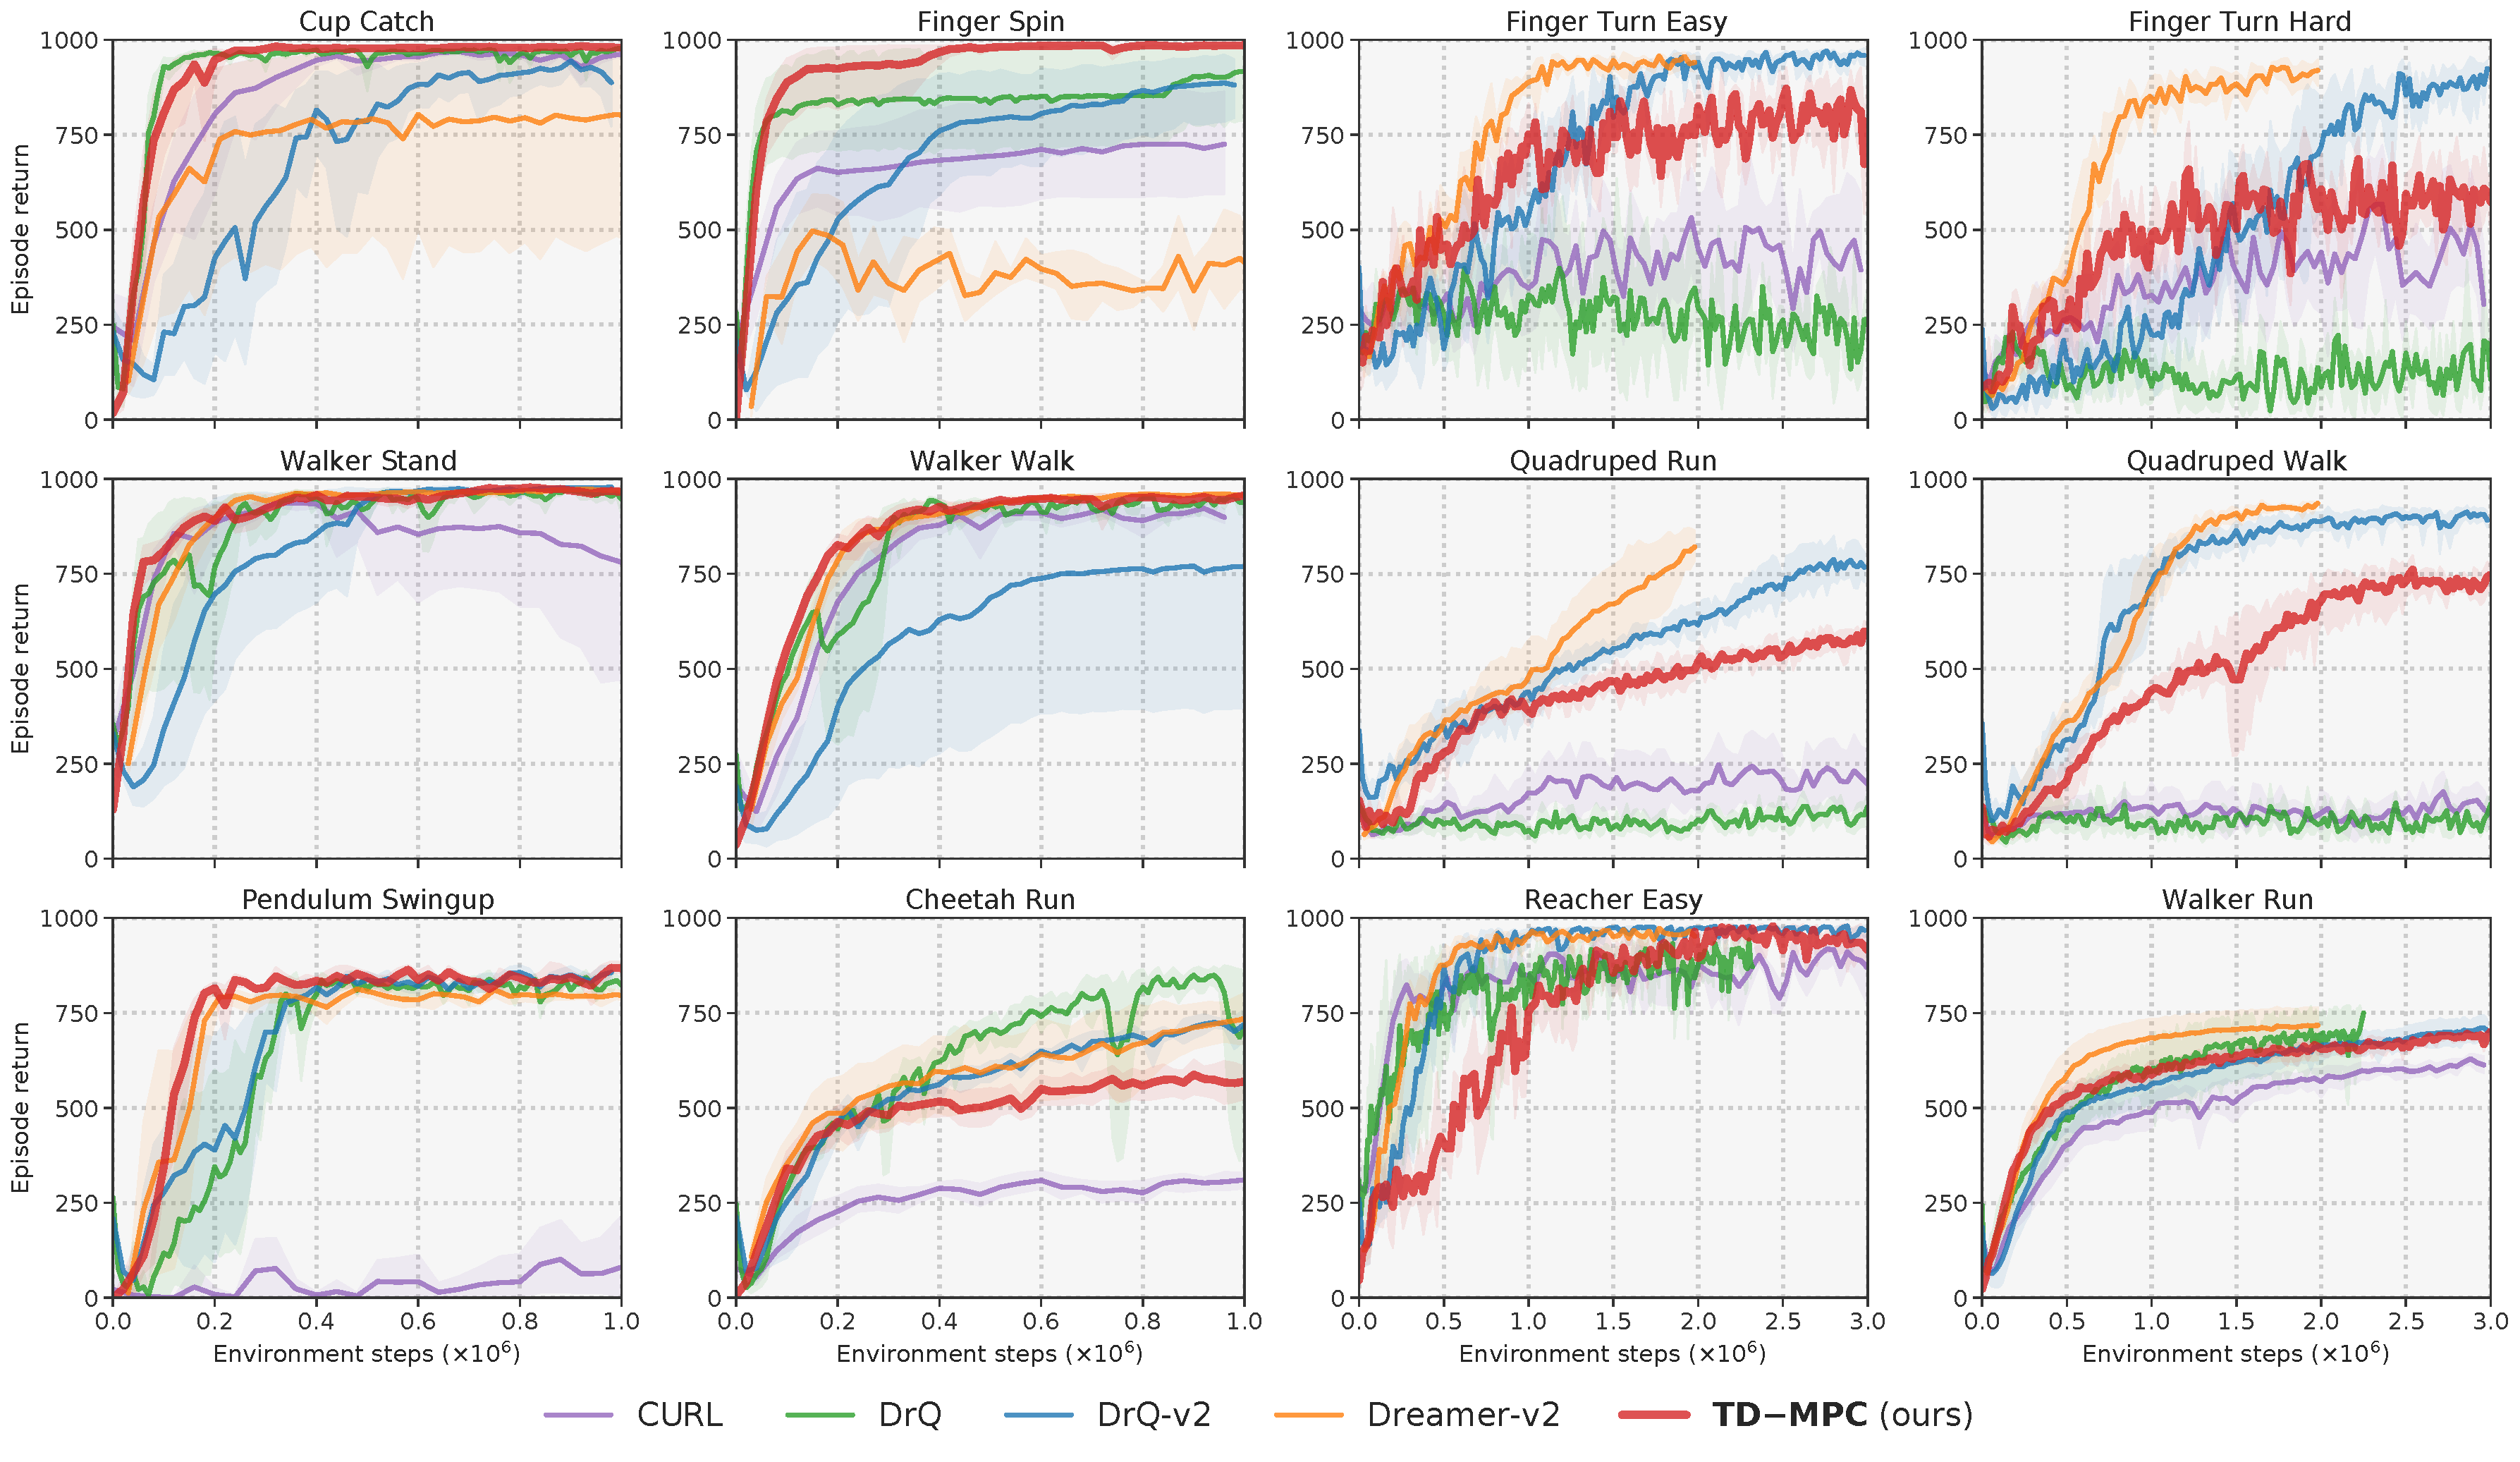
\includegraphics[width=0.88\textwidth]{figures/pixels.pdf}
    \vspace{-0.2in}
    \caption{\textbf{Learning from pixels.} Return of our method (TD-MPC) and state-of-the-art algorithms on 12 challenging image-based DMControl tasks. We follow prior work \citep{Hafner2020DreamTC, hafner2020dreamerv2, yarats2021drqv2} and use an action repeat of 2 for all tasks. Compared to the DMControl 100k benchmark shown in Table \ref{tab:planet}, we here consider more difficult tasks with up to $30\times$ more data. Results for DrQ-v2 and Dreamer-v2 are obtained from \citet{yarats2021drqv2, hafner2020dreamerv2}, results for DrQ are partially obtained from \citet{kostrikov2020image}, and results for CURL are reproduced using their publicly available implementation \citep{srinivas2020curl}. While baselines use task-dependent hyperparameters, TD-MPC uses the \textbf{same} hyperparameters for \textbf{all} tasks. Mean of 5 runs; shaded areas are 95\% confidence intervals. TD-MPC consistently outperforms CURL and DrQ, and is competitive with DrQ-v2 and Dreamer-v2.}
    \label{fig:dreamer}
    \vspace{-0.15in}
\end{figure*}
